\documentclass[]{book}
\usepackage{lmodern}
\usepackage{amssymb,amsmath}
\usepackage{ifxetex,ifluatex}
\usepackage{fixltx2e} % provides \textsubscript
\ifnum 0\ifxetex 1\fi\ifluatex 1\fi=0 % if pdftex
  \usepackage[T1]{fontenc}
  \usepackage[utf8]{inputenc}
\else % if luatex or xelatex
  \ifxetex
    \usepackage{mathspec}
  \else
    \usepackage{fontspec}
  \fi
  \defaultfontfeatures{Ligatures=TeX,Scale=MatchLowercase}
\fi
% use upquote if available, for straight quotes in verbatim environments
\IfFileExists{upquote.sty}{\usepackage{upquote}}{}
% use microtype if available
\IfFileExists{microtype.sty}{%
\usepackage{microtype}
\UseMicrotypeSet[protrusion]{basicmath} % disable protrusion for tt fonts
}{}
\usepackage[margin=1in]{geometry}
\usepackage{hyperref}
\hypersetup{unicode=true,
            pdftitle={Rapport sur l'open data},
            pdfauthor={Samuel Goëta},
            pdfborder={0 0 0},
            breaklinks=true}
\urlstyle{same}  % don't use monospace font for urls
\usepackage{natbib}
\bibliographystyle{apalike}
\usepackage{longtable,booktabs}
\usepackage{graphicx,grffile}
\makeatletter
\def\maxwidth{\ifdim\Gin@nat@width>\linewidth\linewidth\else\Gin@nat@width\fi}
\def\maxheight{\ifdim\Gin@nat@height>\textheight\textheight\else\Gin@nat@height\fi}
\makeatother
% Scale images if necessary, so that they will not overflow the page
% margins by default, and it is still possible to overwrite the defaults
% using explicit options in \includegraphics[width, height, ...]{}
\setkeys{Gin}{width=\maxwidth,height=\maxheight,keepaspectratio}
\IfFileExists{parskip.sty}{%
\usepackage{parskip}
}{% else
\setlength{\parindent}{0pt}
\setlength{\parskip}{6pt plus 2pt minus 1pt}
}
\setlength{\emergencystretch}{3em}  % prevent overfull lines
\providecommand{\tightlist}{%
  \setlength{\itemsep}{0pt}\setlength{\parskip}{0pt}}
\setcounter{secnumdepth}{5}
% Redefines (sub)paragraphs to behave more like sections
\ifx\paragraph\undefined\else
\let\oldparagraph\paragraph
\renewcommand{\paragraph}[1]{\oldparagraph{#1}\mbox{}}
\fi
\ifx\subparagraph\undefined\else
\let\oldsubparagraph\subparagraph
\renewcommand{\subparagraph}[1]{\oldsubparagraph{#1}\mbox{}}
\fi

%%% Use protect on footnotes to avoid problems with footnotes in titles
\let\rmarkdownfootnote\footnote%
\def\footnote{\protect\rmarkdownfootnote}

%%% Change title format to be more compact
\usepackage{titling}

% Create subtitle command for use in maketitle
\newcommand{\subtitle}[1]{
  \posttitle{
    \begin{center}\large#1\end{center}
    }
}

\setlength{\droptitle}{-2em}
  \title{Rapport sur l'open data}
  \pretitle{\vspace{\droptitle}\centering\huge}
  \posttitle{\par}
  \author{Samuel Goëta}
  \preauthor{\centering\large\emph}
  \postauthor{\par}
  \predate{\centering\large\emph}
  \postdate{\par}
  \date{2017-11-26}

\usepackage{booktabs}
\usepackage{amsthm}
\makeatletter
\def\thm@space@setup{%
  \thm@preskip=8pt plus 2pt minus 4pt
  \thm@postskip=\thm@preskip
}
\makeatother

\usepackage{amsthm}
\newtheorem{theorem}{Theorem}[chapter]
\newtheorem{lemma}{Lemma}[chapter]
\theoremstyle{definition}
\newtheorem{definition}{Definition}[chapter]
\newtheorem{corollary}{Corollary}[chapter]
\newtheorem{proposition}{Proposition}[chapter]
\theoremstyle{definition}
\newtheorem{example}{Example}[chapter]
\theoremstyle{definition}
\newtheorem{exercise}{Exercise}[chapter]
\theoremstyle{remark}
\newtheorem*{remark}{Remark}
\newtheorem*{solution}{Solution}
\begin{document}
\maketitle

{
\setcounter{tocdepth}{1}
\tableofcontents
}
\chapter*{Introduction}\label{introduction}
\addcontentsline{toc}{chapter}{Introduction}

A venir

\chapter{Les grands principes d'une démarche d'open
data}\label{les-grands-principes-dune-demarche-dopen-data}

Comme nous allons le voir dans cette première partie, le cadre juridique
de l'ouverture des données repose sur des racines anciennnes mais l'open
data en tant que tel est apparu récemment, il y a moins de 10 ans, avec
des grands principes qui se sont consolidés avec le temps. Dans cette
première partie, nous allons revoir ensemble les grands principes de
l'open data : leurs origines, leur adaptation en France et les bénéfices
pour une collectivité à les adopter.

\section{Aux origines de l'ouverture des données : retours sur quelques
grandes dates
fondatrices}\label{aux-origines-de-louverture-des-donnees-retours-sur-quelques-grandes-dates-fondatrices}

En cinq épisodes, revenons sur les principaux moments de définition des
grands principes internationaux de l'open data. Cette partie permettra
de replacer l'open data dans son contexte d'apparition, de mieux
connaitre les acteurs à l'origine des grands principes et de comprendre
les textes de référence de l'ouverture des données. Nous résumerons les
grands principes de l'ouverture des données dans la partie suivante.

Avant de revenir sur ces différents épisodes, il faut rappeler que le
terme d'open data a des origines plus anciennes que la dernière décennie
sur laquelle nous allons nous concentrer ici. Le terme est apparu pour
la première fois dans les années 1970 dans les accords qu'a signés la
NASA avec des pays partenaires en vue du partage de données
satellitaires. C'est en 1995 qu'on en voit le premier usage public aux
Etats-Unis dans un rapport de la National Academy of Science intitutlé
\emph{On the Full and Open Exchange of Scientific Data}.

\subsection{2005 : Open Definition, la définition juridique des droits
de l'usager du savoir
ouvert}\label{open-definition-la-definition-juridique-des-droits-de-lusager-du-savoir-ouvert}

En août 2005,le chercheur en économie Rufus Pollock, fondateur de l'Open
Knowledge Foundation (OKFN), une organisation à but non lucratif qui
vise à ``~promouvoir l'ouverture de toutes les formes de savoir'',
invitait les premiers membres de l'OKFN et son réseau de partenaires à
adopter collectivement une définition du savoir ouvert. Dans son
\href{https://lists.okfn.org/pipermail/okfn-discuss/2005-August/005233.html}{appel
à commentaire} (\emph{Request for Comments}), Pollock souhaitait
décliner une série de conditions essentiellement juridiques permettant
d'établir qu'un savoir est ouvert. La définition devait aussi servir à
énumérer les licences ouvertes spécifiques au savoir et à fédérer des
disciplines éparses.

Cette définition se fonde directement de l'expérience du mouvement de
l'\emph{open source}, l'ouverture du code informatique, une généalogie
clairement affirmée dans le texte de l'Open Definition qui crédite
l'\emph{Open Source Definition} comme la ressource essentielle qui a
servi à la rédaction de la définition mais aussi à forger l'idée même
d'ouverture. Cet effort de définition s'inscrit aussi dans le
prolongement du travail de Creative Commons qui a défini une série de
licences assorties à des droits et devoirs des usagers d'un savoir
ouvert.

Pour la résumer en quelques mots, l'\href{opendefinition.org}{Open
Definition} quelques années après sa publication) décline les conditions
de l'ouverture du savoir. Cette définition utilise la notion de savoir
pour désigner un domaine très large, qui rassemble des objets
informationnels très différents (donnée, document, contenu, œuvre,
article\ldots{}) Sans entrer dans le détail de chacune des clauses,
l'Open Definition exclut les licences qui «~discriminent~» selon les
types d'usagers ou la finalité de la réutilisation. Elle demande
d'accorder trois droits fondamentaux (utiliser, réutiliser,
redistribuer) et autorise à contraindre les réutilisateurs à deux
exigences possibles~: la citation de la source et le partage des
modifications de l'œuvre avec la même licence (clause de share alike).

En posant la base d'un élargissement de l'\emph{open source} au savoir,
l'Open Definition a constitué une ressource précieuse pour l'ouverture
des données publiques. Elle a établi des critères essentiellement
juridiques qui caractérisent l'ouverture en termes de droits des usagers
sans préjuger du type de savoir concerné. Cet effort de définition s'est
inscrit aussi dans le prolongement du travail de Creative Commons qui a
défini une série de licences assorties à des droits et devoirs des
usagers d'un savoir ouvert.

\subsection{2007 : la rencontre dite de Sebastopol, la définition des
grands principes de l'open
data}\label{la-rencontre-dite-de-sebastopol-la-definition-des-grands-principes-de-lopen-data}

Après avoir découvert les fondements juridiques de l'ouverture des
données avec l'Open Definition, nous partons maintenant aux Etats Unis à
la rencontre de ceux qui ont défini les principes encore aujourd'hui en
vigueur de l'open data.

Le 22 octobre 2007, une invitation est envoyée aux membres d'un groupe
de travail sur l'Open Government pour une rencontre les 7 et 8 décembre
2007 à Sebastopol en Californie au sein des locaux de la maison
d'édition O'Reilly. Les organisateurs de cette rencontre sont Carl
Malamud qui dirige le site associatif \url{PublicRessource.org} et Tim
O'Reilly, le directeur de la maison d'édition O'Reilly spécialisée dans
les sujets technologiques et l'édition électronique ouverte. Dans le
texte de l'invitation, les deux organisateurs se sont fixés pour
ambition de lister dix principes de l'\emph{open government} afin que
les candidats à l'élection du président des États-Unis suivent leurs
recommandations.Trente participants sélectionnés par les organisateurs
en fonction de leur affiliation à une organisation qui demande, ouvre ou
réutilise des données ont accepté l'invitation de Malamud et O'Reilly.

\begin{figure}

{\centering 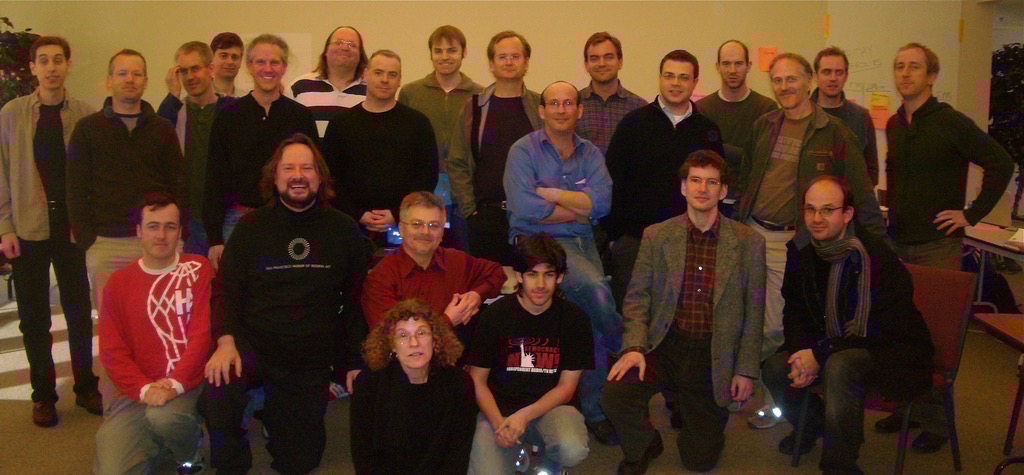
\includegraphics[width=0.7\linewidth]{./img/photofamille} 

}

\caption{La photo de famille des participants de la rencontre de Sebastopol}\label{fig:unnamed-chunk-1}
\end{figure}

Au termes des deux jours de la rencontre de Sebastopol, les participants
ont défini ensemble \href{www.opengovdata.org}{une série de huit
critères} pour que des données gouvernementales soient considérées comme
ouvertes : - \textbf{complètes} : toutes les données publiques doivent
être rendues disponibles dans les limites légales liées à la vie privée
ou la sécurité ;

\begin{itemize}
\item
  \textbf{primaires} : les données ouvertes sont telles que collectées à
  la source, non-agrégées avec le plus haut niveau de granularité ;
\item
  \textbf{fraiches} : les données doivent être disponibles dès qu'elles
  sont produites (\emph{timely}) ;
\item
  \textbf{accessibles} : les données doivent être utilisables par le
  plus grand nombre d'usagers potentiels ;
\item
  \textbf{lisibles par les machines} : les données peuvent faire l'objet
  d'un traitement automatisé par les machines ;
\item
  \textbf{non discriminatoires} : elles peuvent être utilisées par tous
  sans réclamer un enregistrement préalable ;
\item
  \textbf{dans un format ouvert} : ce format ne doit pas être la
  propriété d'une organisation en particulier et doit faire l'objet
  d'une gouvernance commune par ses usagers ;
\item
  \textbf{avec une licence ouverte} : les principes de Sebastopol vont
  plus loin que l'Open Definition en demandant que les données soient
  placées dans le domaine public.
\end{itemize}

Ces principes sont aujourd'hui encore le fondement de l'open data. Les
participants de la rencontre de Sebastopol ont rempli leur objectif, à
savoir l'adoption de ces principes par le futur président des États-Unis
puisque le 21 janvier 2009, jour de son investiture à la Maison-Blanche,
Barack Obama a signé deux mémorandums sur l'\emph{Open Government}. Le
premier exigeait une plus grande coopération des agences
gouvernementales aux procédures du \emph{Freedom of Information Act}
(FOIA). Le second réclamait que les agences gouvernementales mettent en
œuvre des politiques en faveur de la transparence, la collaboration avec
la société civile et la participation des citoyens qui a abouti au
lancement en 2009 de \url{data.gov}, le premier portail open data
national.

\subsection{\texorpdfstring{2008 : ``Raw Data Now'', l'appel du
fondateur du web à l'ouverture des données
brutes}{2008 : Raw Data Now, l'appel du fondateur du web à l'ouverture des données brutes}}\label{raw-data-now-lappel-du-fondateur-du-web-a-louverture-des-donnees-brutes}

Tim Berners-Lee, l'inventeur du web, a formulé son appel à l'ouverture
des données brutes le 4 février 2009 à Long Beach en Californie lors
d'une conférence TED. TED est un réseau de conférences retransmises
gratuitement sur le web qui vise à présenter simplement des idées et à
convaincre l'audience de s'impliquer.

Dans la vidéo de la conférence dépassant aujourd'hui le million de vue,
Tim Berners raconte d'abord son parcours au sein du CERN, l'accélérateur
de particules, où il a développé le web pour facilier le partage des
documents produits dans son laboratoire. Berners-Lee dit ressentir la
même difficulté pour accéder aux données qu'à l'époque de la création
avec les documents. Pourtant, les données déterminent une grande partie
de nos vies. Il se félicite de la naissance de l'open data et des
engagements pris par le président Obama à son arrivée à la Maison
Blanche (son discours est intervenu deux mois après la signature des
mémorandums) mais il estime que l'ouverture des données implique aussi
de transformer les attitudes des administrations.

Pour l'inventeur du web, très souvent, les agents publics sont tentés de
garder leurs données et trouvent une multitude de raisons pour ne pas
les diffuser et permettre leur réutilisation. Dans sa présentation,
Berners-Lee a fait référence au médecin suédois Hans Rosling qui a
proposé l'expression «~\emph{database hugging}~», une métaphore pour
décrire une attitude dans laquelle les agents de l'administration
s'accrochent à leurs données au point de les «~câliner~».Berners-Lee a
repris cette métaphore et l'a mimée sur la scène de TED.

\begin{figure}

{\centering 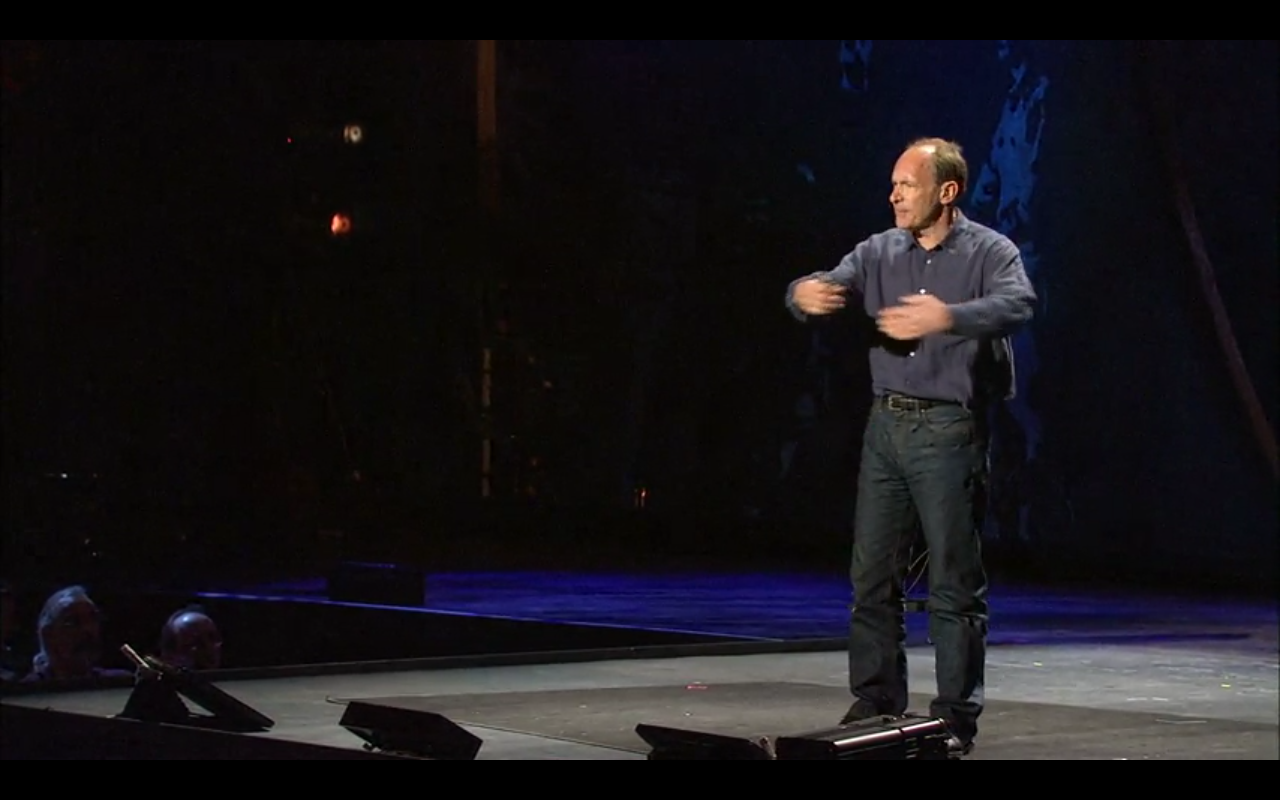
\includegraphics[width=0.7\linewidth]{./img/hug} 

}

\caption{Tim Berners-Lee, lors de sa conférence TED de 2009, mimant le *database hugging*, l’attitude des administrations qui « s’accrochent » à leurs données}\label{fig:unnamed-chunk-2}
\end{figure}

Pour l'inventeur du web, les administrations n'arrêtent le
\emph{database hugging} qu'à partir du moment où elles ont présenté
leurs données sur un beau site web. Il a demandé d'inverser cette
logique et d'abord de fournir les données.

\begin{quote}
Hans appelle ça le * database hugging *. Vous serrez votre base de
données. Vous ne la laissez pas partir tant que vous n'en avez pas fait
un joli site web. {[}\ldots{}{]} Faites-en donc un joli site. Mais avant
cela, donnez-nous accès aux données non altérées. On veut des données.
On veut des données non altérées. \textbf{Il faut que nous demandions
des données brutes maintenant.}
\end{quote}

Tim Berners-Lee demande alors au public de la conférence TED de crier
«~\emph{Raw data now!}~» (``Des données brutes maintenant !'') à
l'attention des administrations.

\begin{figure}

{\centering 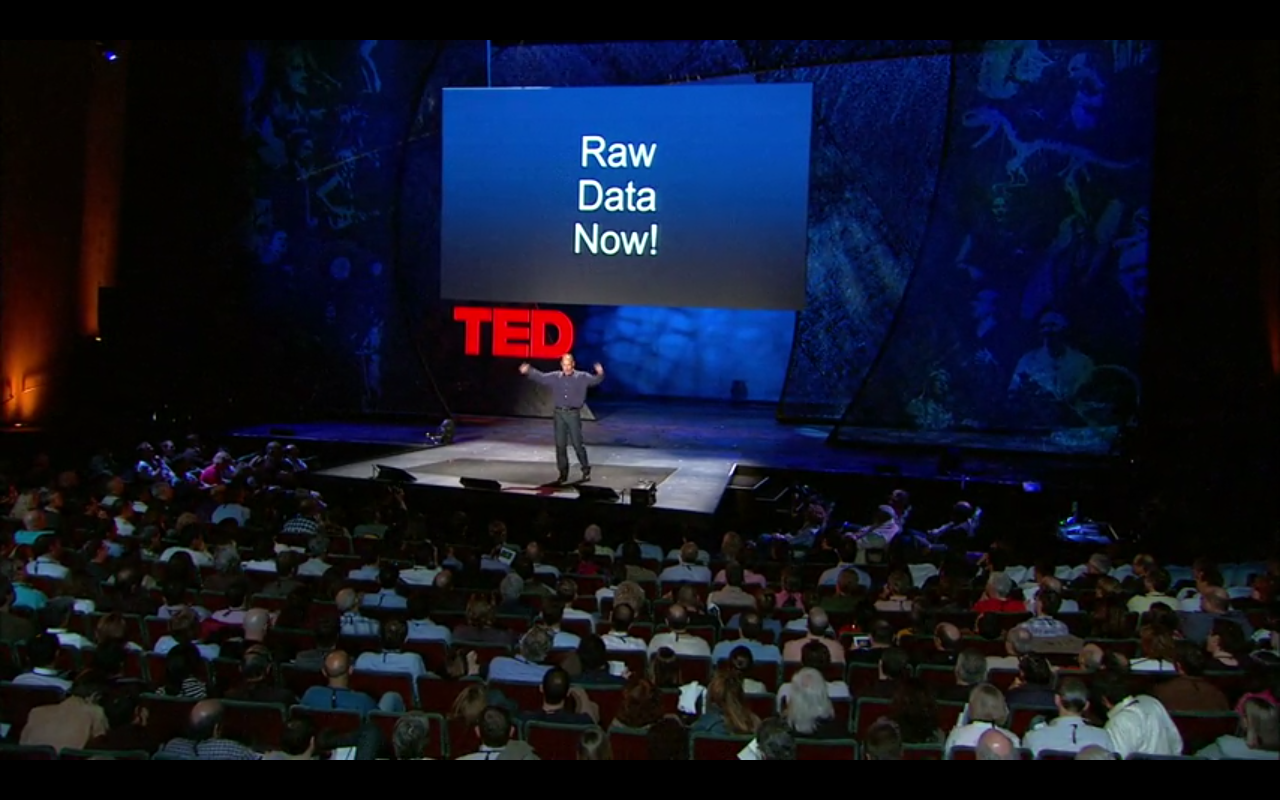
\includegraphics[width=0.7\linewidth]{./img/raw} 

}

\caption{Tim Berners-Lee, lors de sa conférence TED de 2009, Tim Berners-Lee appelle le public à crier « *raw data now* »}\label{fig:unnamed-chunk-3}
\end{figure}

Ce discours de Tim Berners-Lee a imposé la demande de données brutes
comme un aspect essentiel de l'\emph{open data} avec un slogan
facilement mémorable : ouvrez les données brutes maintenant ! Cette
demande de données brutes s'explique par deux choses. D'une part, en
ouvrant les données telles qu'elles sont produites, les administrations
n'auraient pas à les retravailler ce qui a été pensé comme un levier
pour faciliter l'ouverture. D'autre part, l'obtention des données brutes
est pensé comme un moyen de réduire les asymétries d'information entre
l'administration et la société civile puisque les données brutes
seraient le matériau de l'information publique avec son traitement par
l'administration.

\subsection{2010 : le modèle en 5 étoiles, une échelle de l'ouverture
des
données}\label{le-modele-en-5-etoiles-une-echelle-de-louverture-des-donnees}

Après avoir exigé l'ouverture des données brutes, Tim Berners-Lee a
appelé à l'utilisation de formats ouverts de données. En 2010, il
propose un modèle en cinq étapes, une hiérarchie de la première à la
cinquième étoile qui, à la manière de la classification des hôtels,
permet aux réutilisateurs de distinguer la qualité des données. Ce
modèle s'adressait particulièrement aux gouvernements pour les
encourager à adopter le Linked Data pour ouvrir leurs données.

Sur la \href{http://www.cafepress.com/w3c_shop.597992118}{boutique en
ligne du W3C}, le consortium en charge des standards du web, Berners-Lee
vend même des tasses sur lesquelles figure son modèle en cinq étoiles.
Il a déclaré espérer que la circulation de ces tasses dans les bureaux
inciterait à ouvrir et lier toujours plus de données.\\

\begin{figure}

{\centering 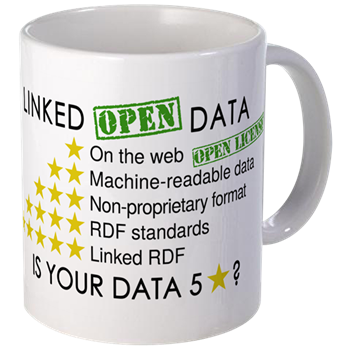
\includegraphics[width=0.7\linewidth]{./img/mug} 

}

\caption{Tasse du W3C reprenant le modèle en cinq étoiles de Tim Berners-Lee.}\label{fig:unnamed-chunk-4}
\end{figure}

Dans la hiérarchie de Tim Berners-Lee, les données sont ouvertes dès la
validation du premier critère. Il considére que, plus une donnée obtient
d'étoiles, plus elle sera simple à utiliser : - ⭐la première étoile
demande la publication sur le web des données, quel que soit leur format
avec une licence ouverte. - ⭐⭐la deuxième étoile exigeant que les
données publiées sur le web sous une licence ouverte soient lisibles par
les machines et structurées. - ⭐⭐⭐la troisième étoile réclame la
publication des données dans un format non propriétaire. - ⭐⭐⭐⭐pour
obtenir la quatrième étoile, les données doivent être publiées dans les
standards ouverts du W3C (RDF et SPARQL) qui imposent que les objets
contenus dans les données soient décrits. ⭐⭐⭐⭐⭐la cinquième étoile
demande qu'elles soient liées à d'autres données publiées sur le web.

Dans les projets d'open data, le modèle de Tim Berners-Lee a été employé
essentiellement pour inciter les agents à ouvrir les données dans des
formats ouverts comme le CSV plutôt que d'utiliser le format Excel.
L'utilisation de formats sémantiques, les deux derniers niveaux du
modèle, réclame un travail trop important de transformation des données
au regard des moyens généralement alloués aux projets d'\emph{open
data}.

Retenons donc du classement en cinq étoiles qu'il suggère aux
administrations d'ouvrir les données de manière progressive. En quelque
sorte, il leur propose une marche à suivre~: d'abord publier les données
sur le web avec une licence ouverte, ensuite avec des formats lisibles
par les machines puis dans des formats ouverts et enfin éventuellement
selon les standards du Linked Data.

\subsection{2013 : la charte internationale de l'open data, vers
l'ouverture par
défaut}\label{la-charte-internationale-de-lopen-data-vers-louverture-par-defaut}

Les 17 et 18 juin 2013 à Loughe-Erne en Irlande du Nord, le Premier
ministre britannique, David Cameron, accueillait la réunion du G8, la
rencontre de huit chefs d'État parmi les plus grandes puissances
économiques mondiales (Allemagne, Canada, États-Unis d'Amérique, France,
Royaume-Uni, Italie, Japon, Russie). Les journalistes en ont
essentiellement retenu les déclarations autour de la Syrie et de la
lutte contre l'évasion fiscale. David Cameron entendait pourtant faire
de Loughe-Erne le «~sommet de la transparence.~» L'agenda comportait une
session (figure \textless{}\$n:figure:G8\textgreater{}) sur la
publication d'information sur les industries extractives, la
transparence de la propriété des terres et l'adoption d'une charte sur
l'\emph{open data}.

 Figure \textless{}\$n:figure:G8\textgreater{}. Une session de travail
des chefs d'État lors du G8 de 2013{[}1{]}.

Contrairement aux cas précédents, je n'ai pas eu accès à des
informations sur les coulisses de ce sommet et de la rédaction de la
charte. Toutefois, j'ai été impliqué au sein de l'OKFN dans la
préparation de l'Open Data Index en vue du G8. L'OKFN était un des
experts techniques sollicités dans la préparation du G8. La charte sur
l'\emph{open data} du G8 se compose d'une série de cinq principes et
trois annexes. La charte part du constat que l'\emph{open data} (nommé
comme tel{[}2{]}) est au cœur d'«~un mouvement mondial~» facilité par la
technologie, les médias sociaux et l'information qui pourra créer de la
croissance économique et rendre les gouvernements plus redevables
(\emph{accountable}) et efficaces. Le préambule détaille les bénéfices
de l'\emph{open data}~: création de services, transparence de l'action
publique, meilleure gouvernance, amélioration du débat public, lutte
contre la corruption, soutien à l'innovation des entreprises et de la
société civile, prospérité renouvelée\ldots{} Pour éviter que
l'\emph{open data} ne soit une «~opportunité manquée~», les chefs d'État
du G8 ont décidé de l'adoption de cinq principes pour régir l'accès aux
données.

Les trois premiers principes établissent les conditions d'ouverture des
données puis les deux derniers fixent deux objectifs~: l'amélioration de
la gouvernance et le soutien à l'innovation. Le premier point de la
charte annonce que les pays signataires s'engagent à faire de
l'\emph{open data} la pratique par défaut des administrations pour les
données publiques tout en respectant les législations en vigueur sur la
propriété intellectuelle et la vie privée. Cette annonce n'engage
toutefois pas les gouvernements qui doivent chacun préciser, d'une part,
leur stratégie d'ouverture des données publiques et, d'autre part,
publier un plan d'action pour mettre en œuvre la charte du G8. L'annexe
technique précise que les gouvernements sont encouragés à publier les
données sur un portail national unique où elles ne pourront être
«~retirées sans préavis.~»{[}3{]} Dans son deuxième principe, la charte
promet la publication de données de qualité. Partant du constat que la
préparation de données exige du temps pour les administrations, elle
propose que les gouvernements se concertent avec des représentants
d'utilisateurs pour définir les données à améliorer en priorité. Les
gouvernements s'engagent à publier les données dès que possible, «~sous
leur forme originale et non modifiée, et au plus fin niveau de
granularité disponible~». Cette dernière demande se rapproche des
exigences de données «~primaires~» des principes de l'\emph{Open
Government Data} ou de données brutes selon Tim Berners-Lee. Selon le
troisième principe, les données doivent être publiées dans des portails
uniques par pays qui n'exigent pas l'enregistrement des utilisateurs.
Elles doivent aussi être gratuites et «~dans des formats ouverts chaque
fois que possible.~» Dans le quatrième principe, les États du G8
s'engagent à partager leur expertise technique avec les pays du monde
entier, notamment au sein d'initiatives multilatérales telles que l'Open
Government Partnership. Ils déclarent vouloir identifier les jeux de
données à ouvrir en priorité avec les organisations de la société
civile. Dans le cinquième principe, les gouvernements s'engagent à
développer la culture de l'ouverture des données («~\emph{increase open
data litteracy}~») et à encourager les organisations de la société
civile qui promeuvent l'\emph{open data}. Dans l'annexe technique, la
charte soutient la publication de données avec une licence libre, mais
n'en fait pas une exigence. Pourtant, tous les acteurs évoqués dans les
épisodes précédents la placent comme une condition essentielle de
l'ouverture des données.

À travers ce résumé, on voit donc que la charte du G8 s'est inscrite
dans la continuité des définitions de l'\emph{open data} évoquées
précédemment. En particulier, elle a repris la majeure partie des
principes de l'\emph{Open Government Data} établis à Sebastopol. Bien
qu'elle ne soit plus au programme des débats du G7, la charte a été
reprise lors d'une rencontre en marge de la conférence internationale
sur l'\emph{open data} qui s'est tenue à Ottawa en mai 2015. La réunion
visait à créer une charte de l'\emph{open data} au-delà des seuls pays
du G8. Elle regroupait des représentants gouvernementaux, des
organisations de la société civile, de plusieurs institutions
internationales et des chercheurs (figure
\textless{}\$n:figure:ottawa\textgreater{}).

 {[}1{]} G8UK sur FlickR, \url{https://www.flickr.com/photos/g8uk/},
consulté le 1 aout 2016. {[}2{]} L'Elysée a traduit open data en
accessibilité des données dans la version complète de la déclaration du
G8 de Lough Erne sur le site de l'Elysée :
\url{http://www.elysee.fr/communiques-de-presse/article/communique-final-du-g/}.
Mais Etalab a publié une version non officielle avec le gouvernement
canadien qui traduit open data en Ouverture des Données Publiques :
{[}3{]} La formulation reprend le principe de permanence établi par la
Sunlight Foundation dans ces dix principes dérivés de l'Open Government
Data.

\section{Revue des grands principes de l'ouverture des
données}\label{revue-des-grands-principes-de-louverture-des-donnees}

\section{Le contexte juridique en
France}\label{le-contexte-juridique-en-france}

\section{Les bénéfices attendus d'une politique d'open data pour une
collectivité}\label{les-benefices-attendus-dune-politique-dopen-data-pour-une-collectivite}

\subsection{Organisationnels}\label{organisationnels}

gain de temps dans les procédures de demandes de données, valorisation
du travail des agents, dialogue avec les citoyens, nouvelles
possibilités de croisement et d'exploitation des données en interne,
possibilité de mutualisation des outils\ldots{}

\subsection{Système d'information}\label{systeme-dinformation}

amélioration de la qualité des données, cartographie du SI, soutien à
l'open source et la souveraineté du SI, possibilité de partage interne
pour les données non ouvrables, avancement de projets de
dématérialisation\ldots{}

\subsection{Communication}\label{communication}

transparence renforcée, visualisation de données pour la communication,
suivi des engagements, implication des citoyens\ldots{}

\subsection{Economie}\label{economie}

soutien aux startups, rationalisation de la politique d'achat par
l'accès à de nouveaux services réutilisant les données, développement
ouvert de services au public par des hackathons et des appels à
projets\ldots{}

\section{Les grands acteurs d'un projet d'open
data}\label{les-grands-acteurs-dun-projet-dopen-data}

\section{En résumé, qu'est-ce qu'une donnée publique ouverte
?}\label{en-resume-quest-ce-quune-donnee-publique-ouverte}

une donnée un document administratif librement réutilisable ouverte
techniquement brute


\end{document}
